\chapter{Exponential Functions}
%%%%%%%%%%%%%%% SECTION HEADER %%%%%%%%%%%%%%%%
\rhead{1}
\lhead{Exponential Functions}
%%%%%%%%%%%%%%%%%%% START %%%$%%%%%%%%%%%%%%%%%
\section{Introduction}
As our study of algebra gets more advanced we begin to study more involved
functions. One pair of inverse functions we will look at are exponential functions
and logarithmic functions. Here we will look at exponential functions and then we
will consider logarithmic functions in another sections.
\section{Exponential functions}
The exponential function is defined by 
\begin{equation}
	f(x) = a^x
	 \label{exp}
\end{equation}
where $a$ is a positive number other than 1 ($a>0$ and $a\neq1$) and $x$ is an real number. The
reason why $a\neq 0,1$ is clear. When $a=0$ or $1$, we will have a horizontal line. \\
On the other hand, it is not straightforward why the base cannot be a negative number. Let's
consider $a=-2$ so that $f(x)=(-2)^x$. Choosing any integer $x-$values yields to another real
numbers. For instance
		\begin{align*}
			f(0) &= 1		&		f(-1) &= -\frac{1}{2} \\
			f(1) &= -2		&		f(-2) &= \frac{1}{4} \\
			f(2) &= 4		&		f(-3) &= \frac{1}{8} \\
				&\vdots		&			&\vdots
		\end{align*}

Here, we don't encounter any problems. However, the graph does not just exist as a set
of these isolated points. The problem arise when $x$ is a fraction such as $0.5$. In this case,
we will get \[
						f(0.5) =(-2)^{0.5} = 1.41i		
			\] 
As it happens, we get a complex number. Likewise, imaginary parts can appear in following $x$
values
		\begin{align*}	
		f(0.75) &= -1.19 + 1.19i \\
		f(1.25) &= -1.68 - 1.68i  \\
		f(1.5) &= -2.83i  \\
		f(1.75) &= 2.38 - 1.38i \\
		\vdots
		\end{align*}
In order to make sense of this, we need to be able to plot these complex $y$ values.
Thus, we need another axis besides the normal $x$ and $y$ axes. Here, we will plot all $x$ values
on the $x$-axis. We then locate the real part of $y$ values on the $y$-axis and their
imaginary part ,if they have any, on the new $z$-axis. The graph of $f(x)=(-2)^x$
is shown in Figure \ref{fig:neg}.
		\begin{figure}[H]
		 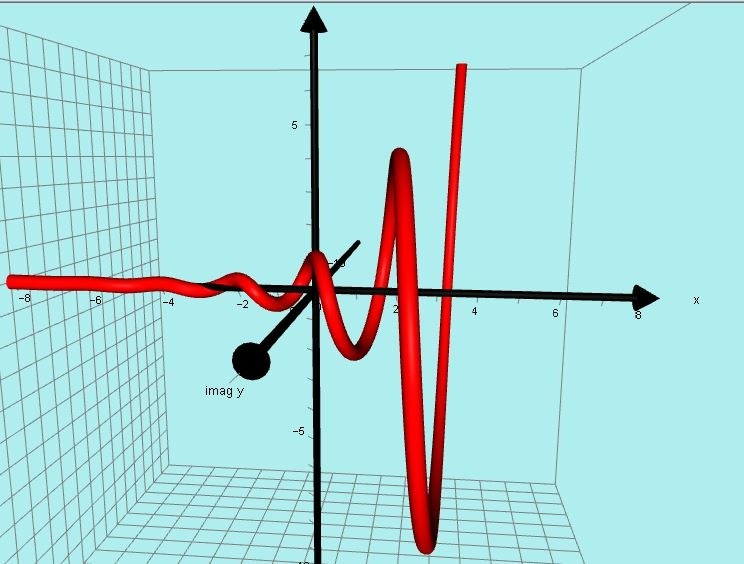
\includegraphics[width=8cm]{pics/neg_base.jpeg}
		 \centering
		 \caption{The graph of $f(x)=(-2)^x$}
		 \label{fig:neg}
		\end{figure}
As you can observe, the negative bases lie beyond the scope of this course. Therefore, we will
only consider positive base other than 1.
\subsection{Exponent rules}
Here are some important algebra rules for exponential functions:
	\begin{align}
		a^0 &= 1	&&\text{Any number to the zero power is equal to 1}\label{zero_exp} \\
		a^{\sfrac{m}{n}} &= \sqrt[n]{a^m} &&\text{Rational notation}	\label{rat_exp}\\
		\left(a^n\right)^m &= a^{nm} &&\text{product rule} \label{prd_exp}\\
		a^{-x} &= \frac{1}{a^x}	&&\text{Negative exponent rule} \label{neg_exp}
	\end{align}
\subsection{Graphing}
It’s really important that you know the general shape of the graph of an exponential function.
There are two options: either the base is greater than 1, or the base is less than 1 (but still
positive).

\subsubsection{Base Greater than 1}
If $a$ is greater than 1, then the graph of $f(x)=a^x$ grows taller as it moves to the right.
Keeping in mind that $a^x$ is positive for any number $x$, and that $a^0  = 1$, we now have a
pretty good idea of what the graph of $f(x) = a^x$ looks like if $a > 1$.
		\begin{figure}[H]
		 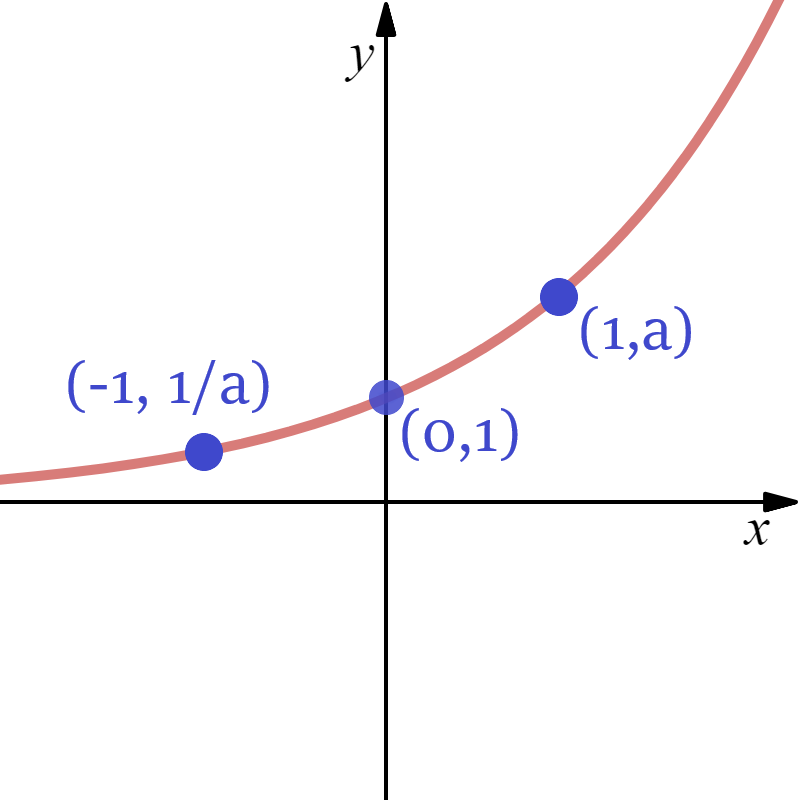
\includegraphics[width=5cm]{pics/a_gt_1.png}
		 \centering
		 \caption{The graph of $f(x)=a^x$ when $a>1$}
		 \label{fig:greater_than_one}
		\end{figure}
As you can see in Figure \ref{fig:greater_than_one}, when moving to the left, the graph becomes shorter and shorter,
shrinking toward, but never touching, the x-axis; In other words, $y=0$ is a horizontal
asymptote. \\
Not only does the graph grow bigger as it moves to the right, but it gets big in a hurry. For
example, if we look at the exponential function whose base is 2, then 
				\[
				f(64)=2^{64}=18,446,744,073,709,525,000
				\]
And 2 isn’t even a very big number to be using for a base (any positive number can be a base, and
plenty of numbers are much, much bigger than 2). The bigger the base of an exponential function,
the faster its graph grows as it moves to the right.\\Moving to the left, the graph of $f(x) = a^x$ grows small very quickly if $a > 1$. Again, if we
look at the exponential function whose base is 2, then
				\[
				f(-10)=2^{-10}=\left(\frac{1}{2} \right)^{10} =\frac{1}{1024}
				\]
The bigger the base, the faster the graph of an exponential function shrinks as it moves to the
left.
\subsubsection{Base less than 1 (but still positive)}
The graph of $f(x) = a^x$ when the base is smaller than 1 slopes down as it moves to the right,
but it is always positive. As it moves to the left, the graph grows tall very quickly. Once
again, the $y$-intercept is at 1 because $a^0$ is always 1. 
		\begin{figure}[H]
		 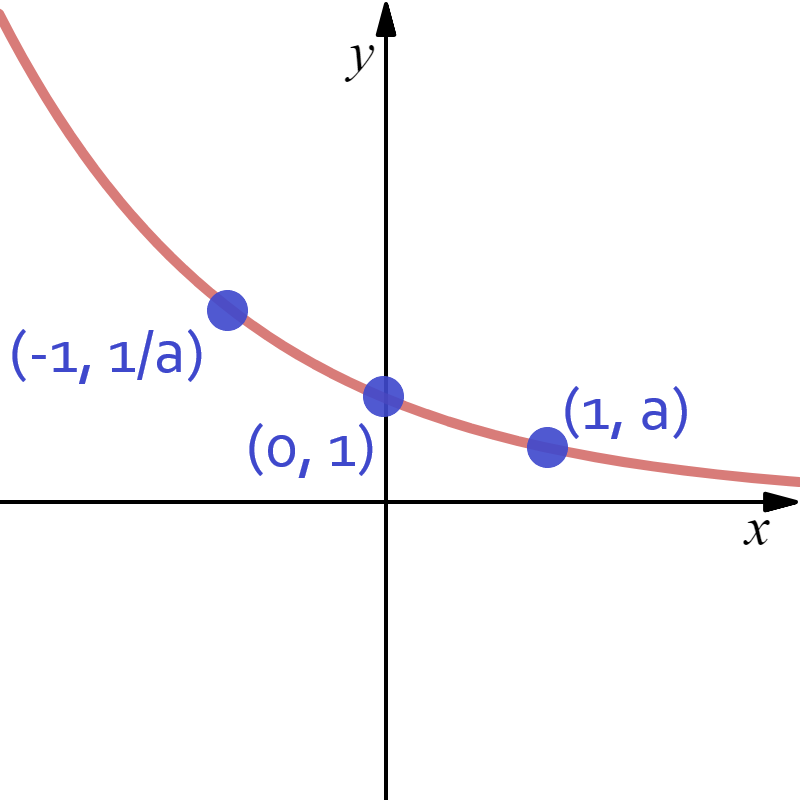
\includegraphics[width=5cm]{pics/a_lt_1.png}
		 \centering
		 \caption{The graph of $f(x)=a^x$ when $0<a<1$}
		 \label{fig:less_than_one}
		\end{figure}
% ============= SUBSECTION
\subsection{One-to-One function}
For any exponential function in the form of $a^x$, domain is all real numbers $(-\infty,+\infty)$. To check what the range of $f(x)$ is, we think of compressing the graph of $f(x)$ onto the $y$-axis. If we did that, we would see that the range of $f(x)$ is the set of all positive numbers, $(0,+\infty)$. \\
We also see from the graph of $f(x) = a^x$, if either $a > 1$ or $0 <a< 1$, $f(x)$ is one-to-one. Remember that to check if $f(x)$ is one-to-one, we can use the horizontal line test (which $f(x)$ passes the test). This means that exponential function has an inverse function; That inverse function is logarithmic function which we will talk about it in later sections. 
\vspace{0.5cm}
	\begin{tcolorbox}[title=Characteristics of $\bm {f(x)=a^x}$, 
	                fonttitle=\bfseries,
	                colframe=red!70!black,
	                colback=white]
	\begin{enumerate}
	\item The domain is $(-\infty,+\infty)$. 
	\item The range is $(0,+\infty)$.
	\item The $y$-intercept is $(0,1)$.
	\item $y=0$ is a horizontal asymptote.
	\item It is a one-to-one function, i.e. it has an inverse.
	\end{enumerate}
	\end{tcolorbox}
% ======= SECTION
\section{\texorpdfstring{$e$}{TEXT}}%
Some numbers are so important in math that they get their own name. One such number is $e$. It is
a real number, but it is not a rational number. It’s very near to – but not equal to – the
rational number 2.7. The importance of the number $e$ becomes more apparent after studying
calculus, but we can say something about it here.

The approximate value of $e$ to nine decimal places is
	\[
		e \approx 2.718281827
	\]
Number $e$ is often called Euler’s Number after \textit{Leonhard Euler}.It is also called Natural Base. 

		\begin{wrapfigure}{r}{0.3\textwidth}
		 \centering
		 
\includegraphics[width=0.25\textwidth]{pics/euler.jpg}
		 \caption{Portrait of \textit{Leonhard Euler}}
		 \label{fig:euler}
		\end{wrapfigure}
%
The discovery of this number is credited to \textit{Jacob
Bernouli} in 1683. He discovered this constant by studying a following question about compound interest:\\ 
%
	“An account starts with \$1.00 and pays 100 percent interest per year. If the interest is
	credited once, at the end of the year, the value of the account at year-end will be \$2.00.
	What happens if the interest is computed and credited more frequently during the year?” \\
%
If the interest is credited twice in the year, the interest rate for each 6 months will be 50\%,
so the accumulated value after one year will be
	\[ 
		\$1.00\times(1.5)^2=\$2.25
    \]
For other compounding we will get
	\begin{align*}
	\$1.00\times(1.25)^4 &= \$2.4414		&	&\text{Compounded Quarterly}\\
	\$1.00\times(1+\frac{1}{12})^{12} &= \$2.613035 & &\text{Compounded Monthly}\\
	\$1.00\times(1+\frac{1}{52})^{52} &= \$2.692597 & &\text{Compounded Weekly}\\
	\$1.00\times(1+\frac{1}{360})^{360} &= \$2.714516 & &\text{Compounded Daily}\\
	&\vdots	&	&\vdots \\
	(1+&\frac{1}{n})^n & &\text{Compounded in $n$ intervals}
	\end{align*}

\textit{Bernoulli} noticed that this sequence approaches a limit with larger $n$. But it was
\textit{Euler} who prove that this expression is approaching a constant number and used the
notation $e$ for this number. He also showed that $e$ is an irrational number and it is equal
to the following beautiful continued fraction 
	\[
		e=2+\cfrac{1}
		  {1+\cfrac{1}
		  {2+\cfrac{1}
		  {1+\cfrac{1}
		  {1+\cfrac{1}
		  {4+\cfrac{1}
		  {1+\cfrac{1}
		  {1+\cfrac{1}
		  {6+\cdots}}}}}}}}
	\]
\subsection{Natural exponential function}	
The natural exponential function is defined by
	\begin{equation}
		f(x)=e^x
		\label{natural}
	\end{equation}

where base is $e$ and $x$ can any real number. Since $e>1$, therefore its graph is increasing.
As you can guess, this function also has a horizontal asymptote $y=0$. Likewise, $(0,1)$ is the
$y$-intercept.  
		\begin{figure}[H]
		 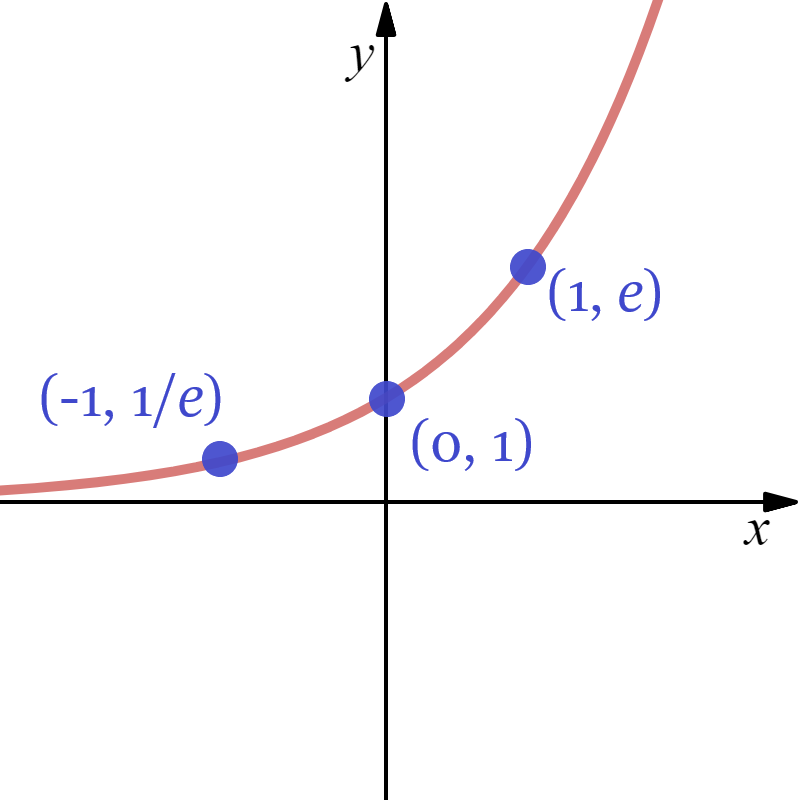
\includegraphics[width=5cm]{pics/natural_func.png}
		 \centering
		 \caption{The graph of natural exponential function}
		 \label{fig:natural_func}
		\end{figure}

\subsection{Compound interest}
One of the application of exponential functions is compound interest. When
money is invested in an account (or given out on loan) a certain amount is added to the
balance. This money added to the balance is called interest. Once that interest is added to the
balance, it will earn more interest during the next compounding period. This idea of earning
interest on interest is called compound interest.

There are several ways interest can be paid. When interest is compounded, one
can calculate the balance after any amount of time using the following formula:
		\begin{equation}
			A=P\left(1+\frac{r}{n} \right)^{nt}
			\label{compounding}
		\end{equation}
where,
		\begin{align*}
			A &: \text{final amount (accumulated value)} \\
			P &: \text{Principal} \\
			r &: \text{Interest rate (as a decimal)}\\
			n &: \text{the number of compounds per year}\\
			t &: \text{time in years}
		\end{align*}
If interest is compounded 
		\begin{multicols}{2}
		\begin{itemize}
			\item annually, then $n=1$
			\item semi-annually, then $n=2$
			\item quarterly, then $n=4$
			\item monthly, then $n=12$
			\item weekly, then $n=52$
			\item daily, then $n=360$
		\end{itemize}
		\end{multicols}
Some banks use continuous compounding, where the number of compounding periods increases
infinitely. When we see the word “continuously” we will know that we cannot use the
formula \eqref{compounding} . Instead we will use the following formula:
		\begin{equation}
			A=Pe^{rt}
			\label{compounding_cont}
		\end{equation}
\begin{exa}
A sum of \$10,000 is invested at annual rate of 8\%. Find the balance in the account after 5
years subject to 
		\begin{enumerate}[a.]
 			\item quarterly compounding;
			 \item and continuous compounding	
		 \end{enumerate}
\end{exa}
We have $P=10,000$, $r=8\%$ which in decimal is $r=\frac{8}{100}=0.08$, and $t=5$ years.
a. In this part, money is compounded quarterly, so $n=4$. Plugging all of these values into
\eqref{compounding} formula, we can find $A$
		\begin{align*}
			A &= P\left(1+\frac{r}{n} \right)^{nt} \\
			A &= \$10,000\left(1+\frac{0.08}{4} \right)^{(4)(5)}\\
			A &= \$10,000\left(1.02 \right)^{20}\\
			A &= \$10,000\left(1.485947 \right)\\
			A &= \$14,859.47
		\end{align*}
b. if money is compounding continuously, then we should use \eqref{compounding_cont}
		\begin{align*}
			A &= Pe^{rt} \\
			A &= \$10,000e^{(0.08)(5)} \\
			A &= \$10,000e^{0.4} \\
			A &= \$10,000(1.4918225) \\
			A &= \$14,918.25
		\end{align*}

As you can observe, the accumulated value of continuous compounding is greater than quarterly
compounding.